% !TeX root = ../main.tex 
\chapter{The HobbySpark interface}
\section{The main window}
The main window of HobbySpark is shown in Fig~\ref{fig:window}.
\begin{figure}[H]
	\centering
	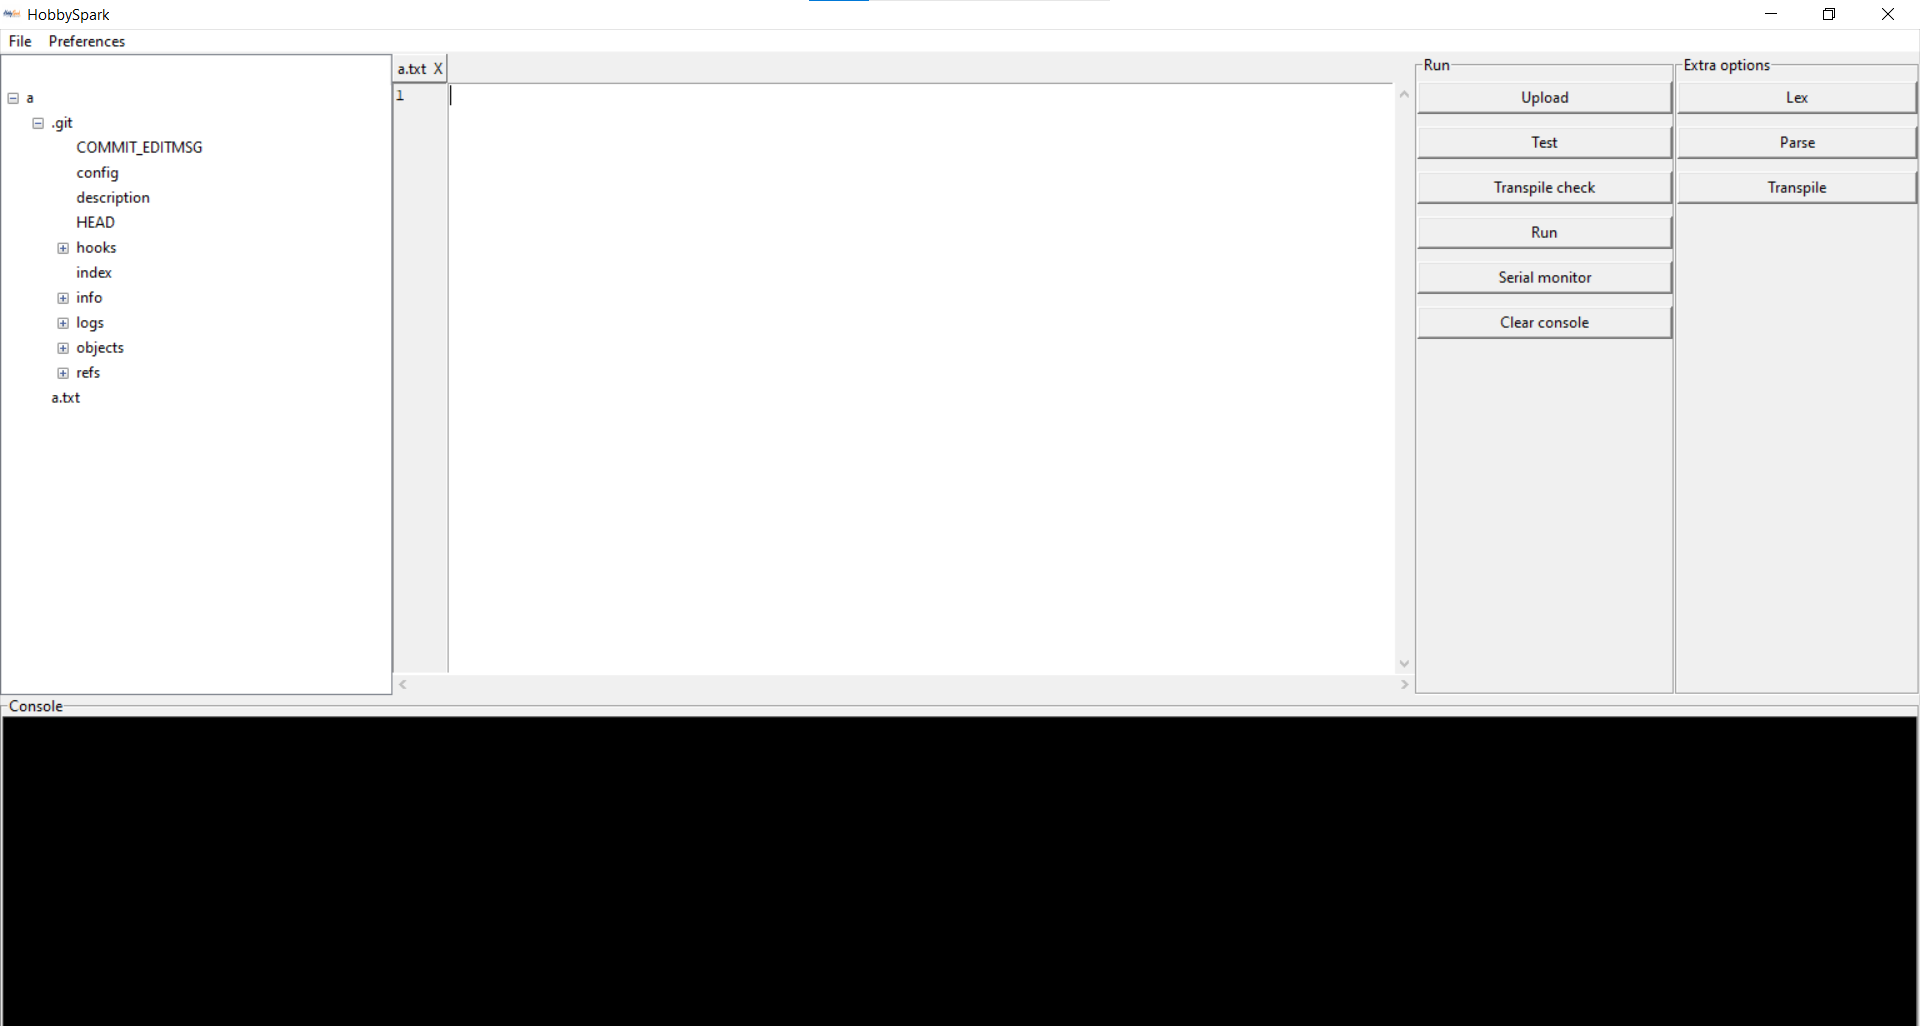
\includegraphics[scale=0.4]{images/main.png}
	\caption{The main window of HobbySpark}
	\label{fig:window}
\end{figure} 




All the buttons and their uses are explained below.

\subsection{Upload}
Uploads the code to the microcontroller, after asking board name and COM port.
\subsection{Test}
Goes through the whole process until compilation; it does not upload. The board name however will be asked.
\subsection{Transpile check}
Tests the program out until transpilation step. Will not ask anything.
\subsection{Run}
Runs the script using the standard \texttt{python filename}. Will not ask anything.
\subsection{Serial monitor}
Opens the serial monitor in a \emph{separate} window, after asking board name, COM port and baudrate.
\subsection{Clear console}
Clears the console.

\subsection{Lex}
Tokenizes the program completely and gives the token list as output for curious users.
\subsection{Parse}
Opens a new window that shows the whole program structure in a tree like structure.
\subsection{Transpile}
Transpiles and shows the complete transpiled C++ code.

\section{Interesting features}
\subsection{Birthday wishing}
\textcolor{red}{YES}, HobbySpark has a builtin birthday wishing system. It features a small window popup and playing of a non-copyrighted "Happy Birthday To You" song.
\subsection{Auto board and COM port fill-up}
Tired of selecting boards and COM ports? Well, fear no more cause we have a file called \texttt{settings.json} in which you can put the default COM port and board. Note that while putting the default values, the value should match exactly to what you get in the drop-down menu, or it may crash unexpectedly.

\section{Menus}
The \texttt{file} menu may be used to create new projects and also open existing ones. A new project in HobbySpark is any folder with the following files/folders:
\begin{itemize}
	\item .src/main.py
	\item COMPILATION/main.py/main.py.ino
	\item COMPILATION/main.py/package.h
	\item settings.json
\end{itemize}


Also note that the COMPILATION directory is auto-generated \emph{after} at least 1 test or upload process has been completed without errors.
\newpage
\section{A note on internal errors}
\begin{figure}[H]
	\centering
	\caption{An internal error that happened} 
	\label{fig:err}
	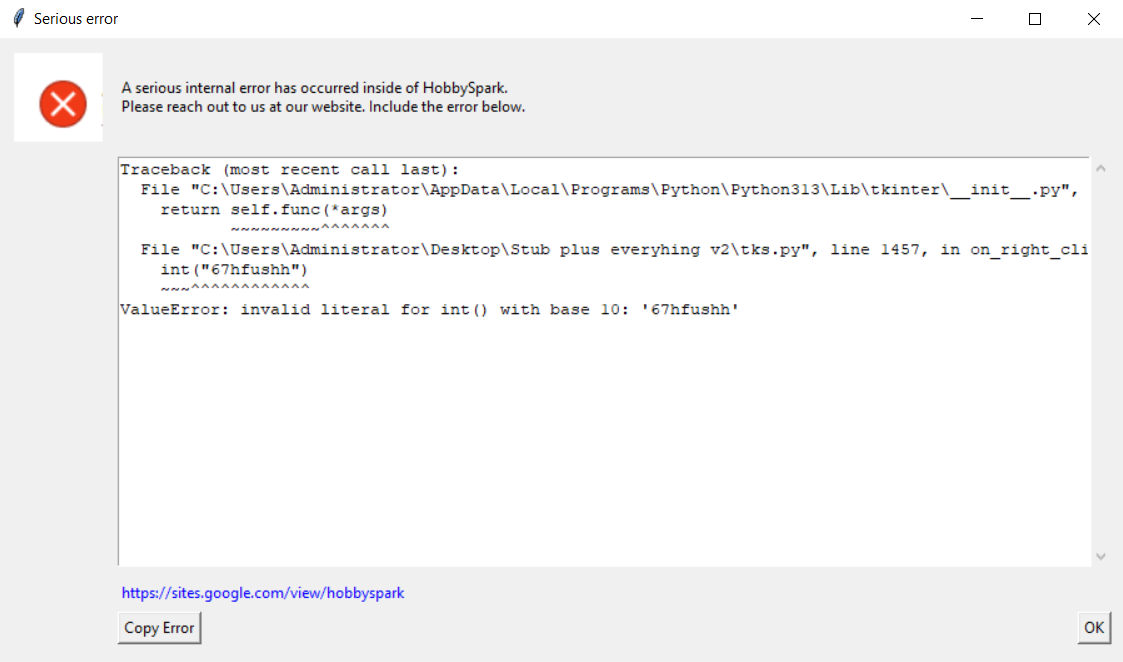
\includegraphics[scale=0.7]{images/error.png}
\end{figure}
While playing around with HobbySpark, if you see something like Fig~\ref{fig:err}, then you should probably do the steps shown on screen. HobbySpark is a developing open-source project. In the first version, the UI may not be stable. Therefore, we have put a safety guard that can watch for errors and report them to the user, so that they can write an issue to us, and we can resolve it.
